\newpage
  \begin{center}
  \section{ }%Как посчитать щели
  \label{sec:_}
  \end{center}
  \begin{figure}[H]
    \centering
    \subfloat[Схема трехкристального эксперимента]{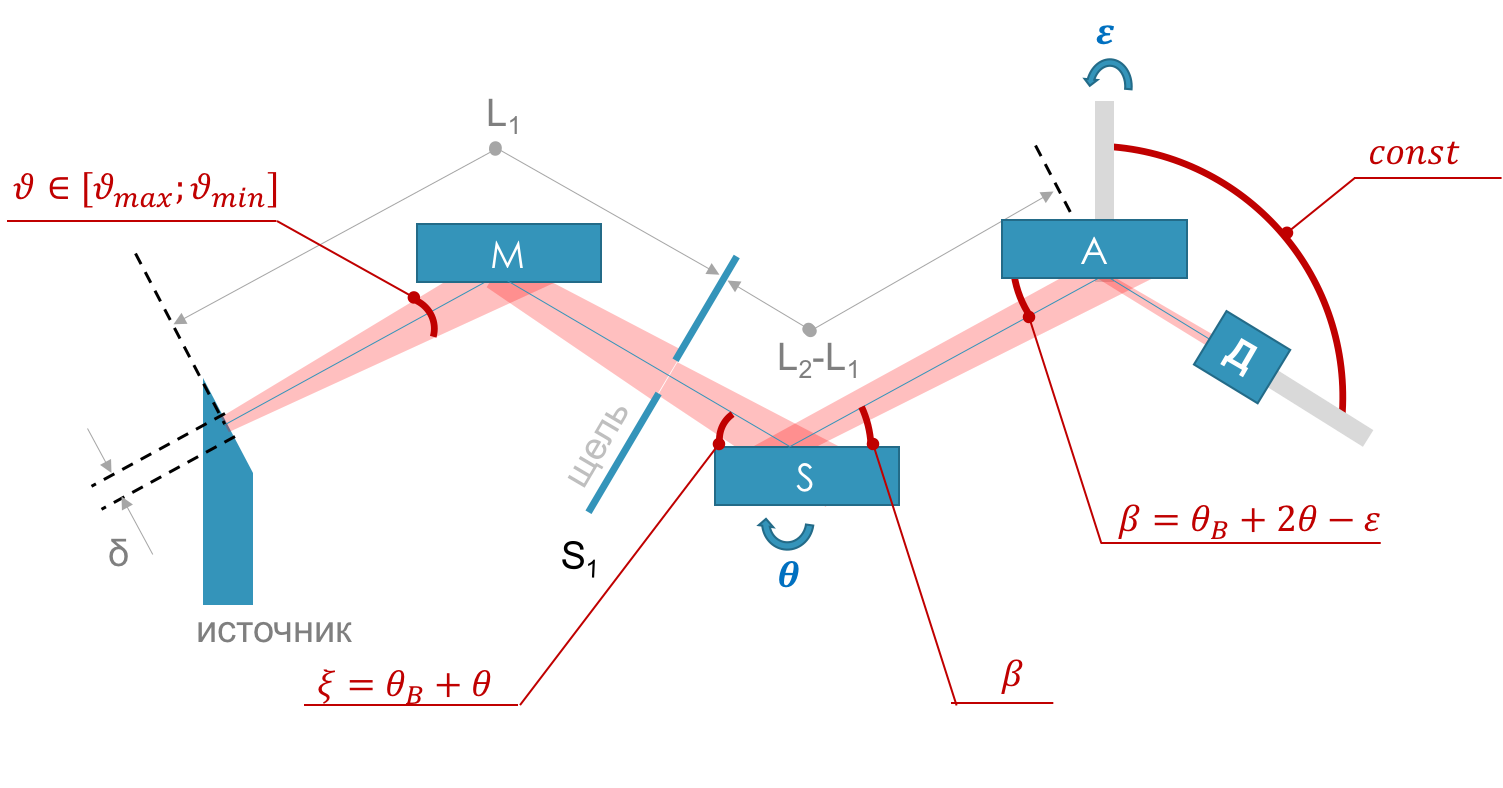
\includegraphics[width=0.65\textwidth]{images/triple_crystal_schem.png}}
    \hfill
    \subfloat[Представление Эвальда]{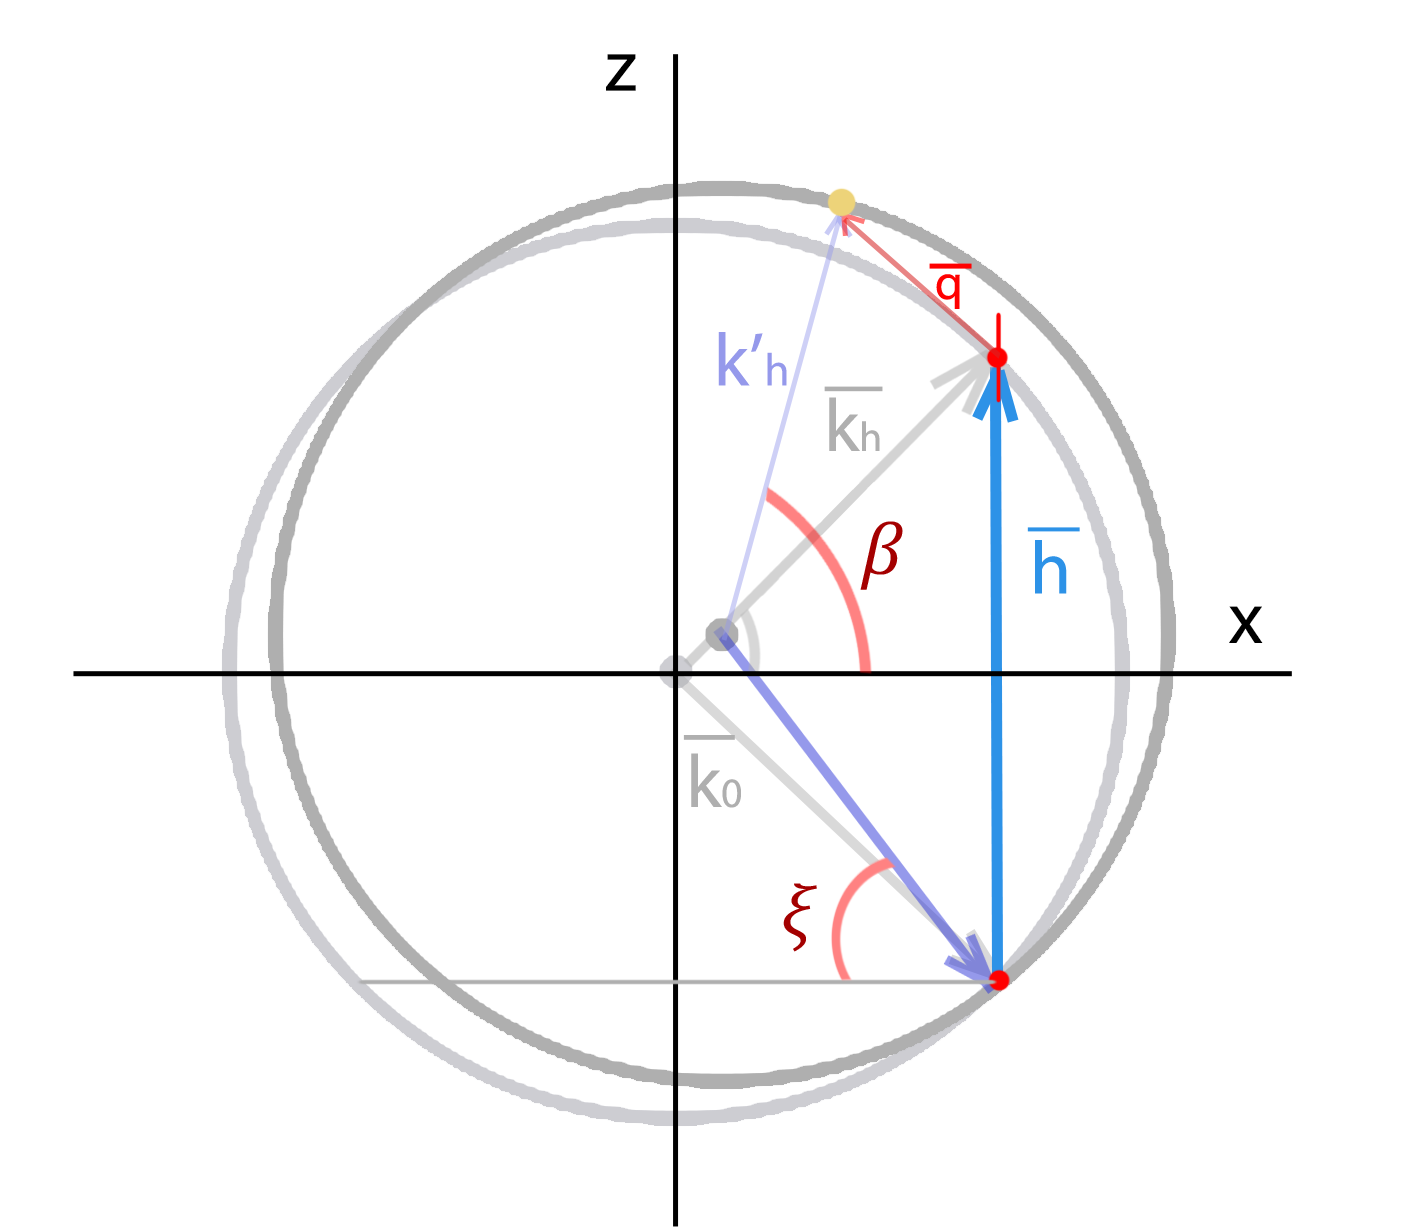
\includegraphics[width=0.35\textwidth]{images/q_vector/ewald.png}}
    \caption{К выводу зависимости между углами поворота элементов схемы и проекциями волновых векторов}
    \label{ris:}
  \end{figure}




  \subsection*{qx}
  \begin{equation}
\label{eqn: distance}
	 q_x/|\vec{k}_0| = cos(\theta_B + \varepsilon -  \theta) - cos(\theta_B +  \theta)
\end{equation}


$$
	  q_x/|\vec{k}_0| =  cos(\theta_B) \cdot cos(\varepsilon -  \theta) - sin(\theta_B)\cdot sin(\varepsilon -  \theta) -
$$

$$
    - cos(\theta_B)\cdot \cancelto{1}{cos(\theta)} + sin(\theta_B) \cdot \cancelto{\theta}{sin(\theta)} =
$$
$$
	 = cos(\theta_B) \cdot [\cancelto{1}{cos(\theta)} \cdot \cancelto{1}{cos(\varepsilon)} + \cancelto{\theta}{sin(\theta)} \cdot \cancelto{\varepsilon}{sin(\varepsilon)}] -
$$
$$
	 - sin(\theta_B) \cdot [\cancelto{\varepsilon}{sin(\varepsilon)} \cdot
	 \cancelto{1}{cos(\theta)} - \cancelto{1}{cos(\varepsilon)}  \cdot
	 \cancelto{\theta}{sin(\theta)}
	 ]  -
$$
$$
	- cos(\theta_B) +  \theta\cdot sin(\theta_B) =
$$
$$
	= cos(\theta_B) + \cancelto{0}{ \theta \cdot \varepsilon \cdot cos(\theta_B) }
	- \varepsilon \cdot sin(\theta_B) +  \theta\cdot sin(\theta_B) - cos(\theta_B) +  \theta\cdot sin(\theta_B)
$$

\begin{equation}
	q_x/|\vec{k}_0| = (2\theta -\varepsilon) \cdot sin(\theta_B)
\end{equation}




\subsection*{qz}
  \begin{equation}
  	q_z/|\vec{k}_0| = sin(\theta_B + \varepsilon -  \theta )+
  	sin(\theta_B + \theta) - 2 sin(\theta_B)
  \end{equation}

  $$
  	q_z/|\vec{k}_0| =   sin(\theta_B) \cdot cos( \varepsilon  -  \theta )+
  	cos(\theta_B) \cdot sin( \varepsilon  -  \theta )+
  	sin(\theta_B) \cdot \cancelto{1}{cos(\theta)}  +
  $$
  $$
  	+cos(\theta_B) \cdot\cancelto{\theta}{sin(\theta)} - 2sin(\theta_B) =
  $$
  $$
  	=  sin(\theta_B) \cdot [\cancelto{1}{cos(\theta)} \cdot \cancelto{1}{cos(\varepsilon)} +\cancelto{\theta}{sin(\theta)} \cdot \cancelto{\varepsilon}{sin(\varepsilon)}
  	]+
  $$
  $$
  	+cos(\theta_B) \cdot [\cancelto{\varepsilon}{sin(\varepsilon)} \cdot
  	 \cancelto{1}{cos(\theta)} - \cancelto{1}{cos(\varepsilon)}  \cdot
  	 \cancelto{\theta}{sin(\theta)}
  	 ]+
  $$
  $$
  	+sin(\theta_B) + \theta \cdot cos(\theta_B)  - 2sin(\theta_B) =
  $$
  $$
  	= sin(\theta_B) +\cancelto{0}{  \theta \cdot \varepsilon \cdot sin(\theta_B)} +			\varepsilon  \cdot  cos(\theta_B)  - \theta  \cdot  cos(\theta_B) +
  $$
  $$
  	+sin(\theta_B) + \theta  \cdot  cos(\theta_B)  - 2sin(\theta_B)
  $$

  \begin{equation}
  	q_z/|\vec{k}_0| = \varepsilon  \cdot  cos(\theta_B)
  \end{equation}
